\section{Prototipa realizācija}

\fixme{This is just random text right now.}

Lai ilustrētu šādas transformāciju sistēmas izstrādes iespējamību, tika izstrādāts sakrišanu meklēšanas mehānisma prototips. Šī nodaļa apraksta prototipa vispārīgās īpašības un pieejas, kas tika lietotas tā realizācijā. Prototips vienkāršības un izstrādes ātruma dēļ tika rakstīts Python valodā, kas ir skriptu valoda, un tāpēc prototips ir viegli palaižams un atkļūdojams uz jebkuras mašīnas ar uzstādītu 2.7.0 Python versiju.

Šīs nodaļas apakšnodaļa~\ref{subsec:solution_problems} savukārt apraksta problēmas ar kurām saskārās darba autors un izņēmumus, kas pagaidām netiek implementēti prototipā.

\fixme{Pārrakstīt atkarībā no satura}

\subsection{\label{subsec:solution_syntax}Atļautā makro sintakse}

Kā jau bija pateikts, makro pieejamā regulāro izteiksmju sintakse ir minimāla. Tā atļauj lietot \verb|*| lai identificēt tokenu virknes un \verb/|/ lai izvēlēties starp dažiem tokenu tipiem.

Prototips arī ļauj veidot regulārās izteiksmes ar specificētu tokenu vai pseido-tokenu vērtībām. Piemēram, regulārā izteiksme \verb|{id:foo}| sagaidīs tieši identifikatoru \verb|foo|, bet izteksme \verb|{id}| sagaidīs jebkuru identifikatoru.

\subsection{\label{subsec:solution_approach}Vispārīgā pieeja}
Šī apakšnodaļa vispārīgi apraksta sistēmas prototipa darbību virkni.

Prototips imitē darbu reālajā vidē, saņemot pa vienam tokenus no ieejas plūsmas. Tokenu plūsmas saskarne imitē leksera darbu. Kamēr prototips nav saņēmis nevienu regulāro izteiksmi, tas ignorē tokenu plūsmas apstrādes izsaukumus. Tiklīdz prototipam tiek padota tokenu regulārā izteiksme, tas uzsāk regulārās izteiksmes parsēšanu. Parsēšanas procesā tiek izveidots galīgs automāts, kas akceptē regulārās izteiksmes uzdotās virknes.

Tad, kad atnāk tokenu apstrādes pieprasījums, sistēma izpilda pārejas starp automātu stāvokļiem, meklējot sakrišanas, un atceras tokenus, kurus jau ir nolasījusi. Sistēma atrod garāko virkni, kas atbilst kādam no šabloniem un tad atgriež tās identifikatoru un nolasīto tokenu virkni, lai turpmāk transformēšanas mehānisms varētu pārstrādāt to jaunajā virknē.

Pieņemot, ka transformēšanas sistēma ir izstrādāta, tālākā darba gaita būs sekojoša. Transformēšanas sistēma aizstāv ielasīto virkni ar citu, kas ir konstruēta pēc akceptētās regulārās izteiksmes noteikumiem. Tad sakrišanas meklēšanas sistēmas darbs tiek uzsākts no aizvietotās virknes sākuma.

Sistēma turpina darbu aprakstītā gaitā līdz ko neviens no šabloniem vairs netiek akceptēts. Pēc sistēmas apstāšanās tiek iegūta jauna tokenu virkne, kas tika apstrādāta attiecīgi kodā ierakstītiem makro. Kad sistēma tiks integrēta ar reālu kompilatoru, tā strādās paralēli ar parsētāju un sistēmas izejas tokenu virkne tiks apstrādāta ar standartiem valodas likumiem.

\subsection{\label{solution_conflictresolving}Makro konfliktu risināšana}
Makro šablonu konflikti var rasties tad, kad daži makro var tikt akceptēti vienlaikus. Tas var notikt gadījumos, ja divas regulārs izteiksmes akceptē līdzīgas virknes. Zemāk tiks aprakstīts, kā tika izvēlēts risināt dažādas konfliktu situācijas. 

Reālajā situācijā var rasties 3 konfliktu veidi. Pirmais var rasties gadījumā, ja divas izteiksmes atpazīst vienu un to pašu virkni vienā tvērumā. Otrais var rasties gadījumā, ja jaunajā tvērumā parādās šablons, kas ir līdzīgs jau eksistējošam šablonam no vispārīgāka tvēruma. Trešais var rasties tad, kad viena no izteiksmēm akceptē kādu virkni, bet cita akceptē garāku virkni.

\subsubsection{Divu makro konflikts vienā tvērumā.}

Gadījumā, ja viena tvēruma ietvaros eksistē divi šabloni, kas dod sakritību ar vienādu garumu, tad tiek ņemtas vērā prioritātes. Tā izteiksme, kas tika ielasīta agrāk būs ar lielāku prioritāti nekā tā, kas ir ielasīta vēlāk. Tātad ja secīgi tiks ielasītas divas izteiksmes \verb|{id} {(} {)}| un \verb|{id} {(} ( {real} * ) {)}|, tad ielasot virkni \verb|{id:foo} {(} {)}| tiks akceptēta pirmā izteiksme. Gadījumā, ja izteiksmes tiks ielasītas pretējā secībā, pirmā izteiksme nekad netiks atpazīta, jo otrā izteiksme pārklāj visas pirmās izteiksmes korektās ieejas.

\subsubsection{Divu makro konflikts dažādos tvērumos.}

Tvēruma iekšienē strādā tādi paši likumi par izteiksmju prioritātēm - izteiksme, kas bija agrāk ir ar lielāku prioritāti. Bet makro, kas ir specifiski tvērumam ir ar lielāku prioritāti nekā vispārīgāki makro. Tātad, ja pirmajā tvērumā tiks ieviestas makro \verb|1| un \verb|2|, bet otrajā tvērumā tiks ieviestas marko \verb|3| un \verb|4|, to prioritāšu rinda izskatīsies sekojoši: \verb|3, 4, 1, 2|. Pirmie makro ir ar lielāku prioritāti, nekā tie, kas atnāca vēlāk, bet vēlāka tvēruma makro ir ar lielāku prioritāti neka tie, kas atrodami agrākā tvērumā.

\subsubsection{Dažādu virkņu garumu konflikts}
Prototips strādā pēc $greedy$ principa - tas akceptē visgarāko iespējamo šablona sakritību. Tātad, ja eksistē divi šabloni \verb|{int} {,}| un \verb|({int} {,}) *|, tad tokenu virkne \verb|{int:4} {,} {int:6} {,}| tiks akceptēta ar otru šablonu, neskatoties uz to, ka augstākās prioritātes šablona sakritība tika konstatēta agrāk.

\subsection{\label{subsec:solution_motivation}Realizācijas pamatojums}

Galvenais princips prototipa risinājuma izstrādē bija izveidot to tā, lai jebkurā laika momentā šablonu sakrišanu meklēšanai būtu nepieciešams lineārs laiks un tikai viena pāreja pa tokenu virkni. Šāda pieeja ir izvēlēta ar iedomu, ka makro pievienošana tiks izpildīta tikai vienreiz, bet sakrišanu meklēšana tiks pildīta katrā produkcijā, un, sliktākajā gadījumā, katram tokenam no ieejas plūsmas.

Ielasītās regulārās izteiksmes tiek pārsētas un pārveidotas nedeterminēta galīgā automātā. Tad katrs no nedeterminētiem galīgiem automātiem tiek determinizēts un minimizēts. Tātad katrai regulārai izteiksmei tiek izveidots minimāls determinēts automāts, kurš ir optimizēts gan pēc laika, gan pēc aizņemtās vietas.

Tālāk, lai nodrošinātu visu šablonu pārbaudi, ir nepieciešams apvienot izveidotos automātus. To var izdarīt dažos veidos. Vienkāršākais no tiek būtu glabāt visus galīgos automātus sarakstā. Pieņemsim, ka ir $n$ šabloni, kurus vajag pārbaudīt. Tad automātu saraksts reprezentē nedeterminētu galīgu automātu ar $n$ $\varepsilon$-zariem no sākuma stāvokļa, katrs no kuriem ved pie sākuma stāvokļa vienam no jau izveidotiem determinētiem automātiem.

Cits veids, kā to varētu izpildīt, ir apvienot visus izveidotos šablonu automātus vienā determinētā galīgā automātā. Tieši šīs veids tika izvēlēts šī darba ietvaros lai pēc iespējas samazinātu laiku sakrišanu meklēšanai. Kaut arī automātu apvienošana šādā veidā ir laikietilpīga, tā samazina laika kārtu sakritību meklēšanai. Šāda izvēle ir balstīta uz faktu, ka makro daudzums būs samērā neliels, bet gan sakrišanu meklēšanas izsaukums var notikt katras produkcijas ietvaros, t.i. katra tokena apstrādē.

Diemžēl pilnībā lineāra laika sakrišanu meklēšana nav iespējama tādēļ, ka prototips dod iespēju lietot makro ar tokenu vērtībām. Piemēram, eksistē 2 makro, viens no kuriem vēlās saņemt tokenu \verb|{id}|, un otrs \verb|{id:foo}|. Gadījumā, kad sakrišanu meklēšanas procesā parādās tokens \verb|{id:foo}|, automātam nav iespējas izsecināt, kurš no ceļiem novedīs pie garākas sakritības. Tādēļ tas iet pa abiem ceļiem vienlaikus, saglabājot abus stāvokļus.

Automātu minimizēšana ir diezgan darbietilpīga operācija (sk.~\ref{subsubsec:prototype_minimization}), tāpēc tā tiek izpildīta tikai uz atsevišķiem automātiem. Liels automāts nebūs minimāls, jo dažādu minimālu automātu apvienošana negarantē šo faktu, bet tā kā apvienota automāta stāvokļu daudzums var būt ļoti liels, minimizēšanas izpilde var būt neefektīva. Tā kā minimizēšana samazina tikai automāta aizņemto vietu, nevis apstaigāšanas laiku, to var neieverot.

\subsection{Kāpēc neder jau uzrakstītas bibliotēkas}

Šinī darbā aprakstītai apstrādei neder jau izstrādātas regulāro izteiksmju bibliotēkas, kaut arī ir izstrādātas daudzas bibliotēkas, gan parastās, gan ar līdzīgu pieeju, ko apskata šīs darbs (piem.~\cite{RE2}, kas lieto automātu teoriju lai paātrinātu apstrādes laiku). Tās neder tādēļ, ka regulāro izteiksmju dzinēji strādā ar tekstu, nevis ar tokeniem. Tie arī parasti piedāvā daudz vairāk funkcionalitātes, nekā ir nepieciešams, piemēram, meklēšana no virknes sākuma. Citu programmētāju rakstītā koda pārstrāde aizņemtu vairāk laika nekā tā izveidošana pilnīgi no jauna.

Jau eksistējošās bibliotēkas nepiedāvā iespēju apvienot visus automātus viena vienīgā. Eksistējošie apvienošanas risinājumi, savukārt, pēc apvienošanas neņem vērā, tieši kāda regulārā izteiksme uz doto brīdi ir akceptējoša. Šī darba ietvaros šīs informācijas saglabāšana ir būtiska, jo no tās ir atkarīgs, kāda no transformācijām ir lietota. 

Apvienošanas pieeja parasti ir lietota lielu datu plūsmu apstrādē, piemēram, meklējot infekcijas pazīmes plūsmā. Tad izstrādātās regulārās izteiksmes ir optimizētas un apvienotas vienā automāta. Šādā gadījumā nav nozīmes, kura no izteiksmēm ir akceptēta, jo galvenais ir identificēt draudu pazīmes. 

\subsection{\label{subsec:solution_algorithms}Lietotie algoritmi}

Šī apakšnodaļa apraksta pieejas un algoritmus, kas tika lietoti prototipa realizācijā. Kā jau bija teikts, meklēšanas laika optimizācijai tika izvēlēta pieeja, kur visi regulāro izteiksmju automāti tiek sapludināti kopā.

Visu automātu pārejas pa zariem notiek nevis pa kādu simbolu, bet gan pa tokeniem.

\subsubsection{Regulāro izteiksmju pārveidošana nedeterminētā galīgā automātā}

\fixme{Proof that they have the same computational power}

Regulāro izteiksmju translēšana uz nedeterminētu galīgu automātu ir diezgan vienkārša. Ir nepieciešams tikai pārveidot galvenos kontroles elementus. Tā kā uz doto brīdi prototips atbalsta tikai ierobežotu regulāro izteiksmju sintaksi, to ir vienkārši izdarīt.

Nedeterminēts galīgs automāts (NGA) veselai regulārai izteiksmei ir izveidots to daļējiem automātiem katrai regulārās izteiksmes daļai. Katram operatoram tiek piekārtota attiecīga konstrukcija. Daļējiem automātiem nav akceptējošu stāvokļu, tiem ir pārejas uz nekurieni, kuras vēlāk tiks lietotas lai savienotu automāta daļas. Pilnīga automāta būvēšanas process beigsies ar akceptējošā stāvokļa pievienošanu palikušajām pārejām.

NGA vienam tokenam ${token}$ izskatīsies sekojoši:
\begin{figure}[h]
  \centering
    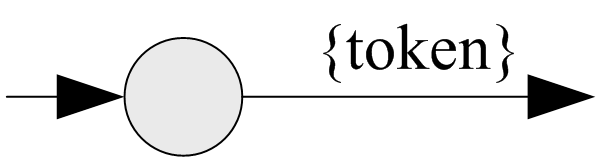
\includegraphics[scale=1.5]{pictures/auto_token_1}
  \caption{\label{fig:auto_token}Automāts vienam tokenam}
\end{figure}

NGA divu automātu konkatenācijai $e_1 e_2$  izskatīsies sekojoši:
\begin{figure}[h]
  \centering
    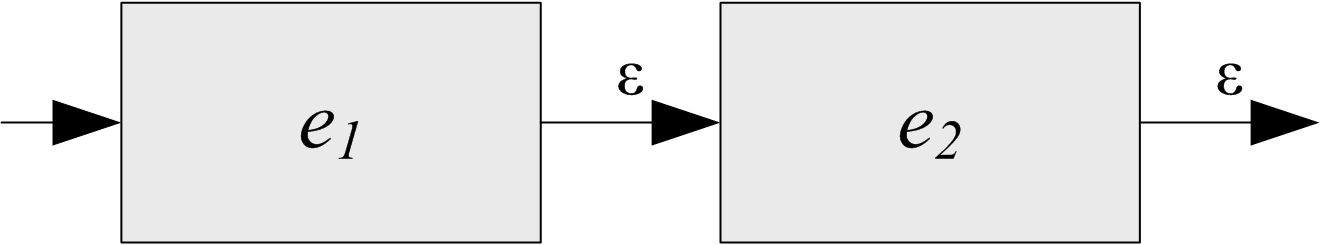
\includegraphics[scale=1.5]{pictures/auto_sequence_1}
  \caption{\label{fig:auto_sequence}Automāts divu automātu konkatenācijai}
\end{figure}

NGA izvēlei starp diviem automātiem $e_1 | e_2$ izskatīsies sekojoši:
\begin{figure}[h]
  \centering
    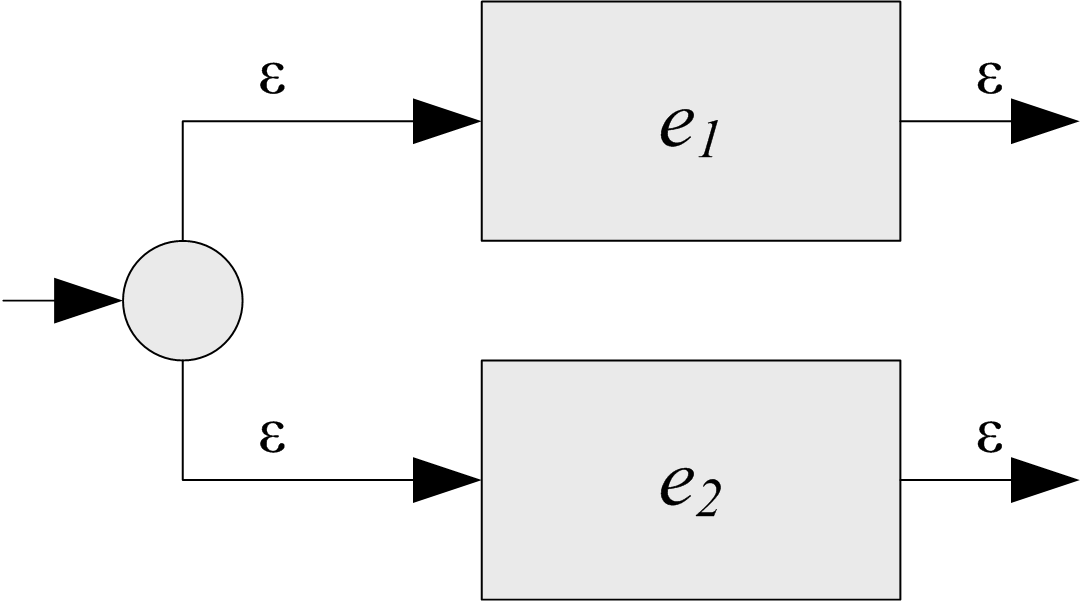
\includegraphics[scale=1.5]{pictures/auto_or_1}
  \caption{\label{fig:auto_or}Automāts izvēlei starp diviem automātiem}
\end{figure}

NGA priekš konstrukcijas $e_1 *$ izskatīsies sekojoši:
\begin{figure}[h]
  \centering
    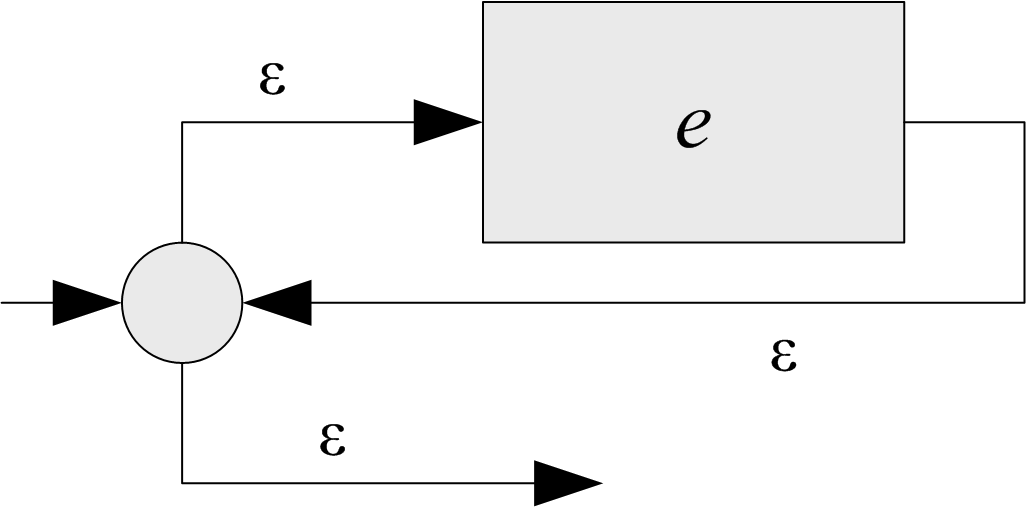
\includegraphics[scale=1.5]{pictures/auto_asterisk_1}
  \caption{\label{fig:auto_asterisk}Automats automātu virknei}
\end{figure}

Tālāk šie automāti tiek apvienoti vienā, piemēram izteiksmei \verb/{id} ({real} | {int}) * {;}/ NGA izskatīsies sekojoši:
\fixme{picture}

Tā tiek izveidots nedeterminēts automāts katrai regulārai izteiksmei. \cite{Cox:RegexpMatchingFast}, \cite{DragonBook}

\subsubsection{Determinizācija}

Kaut arī daudzām valodām ir vienkāršāk uzbūvēt nedeterminētu galīgu automātu (piemēram, pašām regulārām izteiksmēm tas ir loģiskāk), ir patiess tas, ka katra valoda var tikt aprakstīta gan ar nedeterminētu, gan ar determinētu galīgu automātu. Turklāt, dzīvē sastopamās situācijās DGA parasti satur tik pat daudz stāvokļu, cik ir NGA. Sliktākajā gadījumā, tomēr var gadīties, ka mazākais iespējamais DGA saturēs $2^n$ stāvokļu, kamēr mazākais NGA saturēs $n$ stāvokļus. \footnote{Pieņemsim, ka automāta valoda sastāv no diviem simboliem - {0, 1}. Sliktākais gadījums, kad DGA tiešām saturēs $2^n$ stāvokļus attiecībā pret $n$ NGA stāvokļiem, var rasties tad, kad, piemēram, automāta valodā $n$-tais simbols no virknes beigām ir 1. Tad DGA būs jāprot atcerēties pēdējos $n$ simbolus. Tā kā ir divi ieejas alfabēta simboli, automātam ir jāatceras visas to dažādas $2^n$ kombinācijas.}

Izrādās, ka patiesībā katram NGA eksistē ekvivalents DGA, ko var uzbūvēt ar apakškopu sastādīšanas algoritmu (pierādījumu tam, ka uzbūvētais DGA tik tiešām akceptē to pašu valodu, ko NGA, sk.  \cite{Hopcroft:IntroAutomataTheory}, teorēma 2.11.) Vadošā doma šī algoritmā ir tas, ka katrs determinētā galīgā automāta (DGA) stāvoklis ir kādu NGA stāvokļu kopa. Pēc ieejas virknes $a_1, a_2, ..., a_n$ ielasīšanas DGA atrodas stāvoklī, kas atbilst NGA stāvokļu kopai, kuru var sasniegt apstaigājot virkni $a_1, a_2, ..., a_n$.

\paragraph*{Algoritms 1: NGA transformēšana uz DGA}
\subparagraph*{Ieeja}NGA $N$.
\subparagraph*{Izeja}DGA $D$, kas ir ekvivalents $N$.
\subparagraph{Algoritms} Sākumā algoritms konstruē pāreju tabulu priekš $D$. Katrs $D$ stāvoklis ir $N$ stāvokļu kopa, tātad tabula tiek konstruēta tā, lai $D$ simulētu vienlaikus visas pārejas, ko var izpildīt $N$, saņemot kādu ieejas virkni. Lai automāts kļūtu determinēts, ir nepieciešams atbrīvoties no iespējas atrasties dažos stāvokļos vienlaikus. Tātad vajag atbrīvoties no $\varepsilon$-pārejām, un no daudzkārtīgām pārejām no viena stāvokļa pa vienu ieejas simbolu.

Tabulā~\ref{fig:NGAoperations} var redzēt divas funkcijas, kas ir nepieciešamas NGA apstrādes izpildei. Šīs funkcijas no NGA stāvokļiem un pārejām veido jaunas stāvokļu kopas, kuras veidos DGA stāvokļus.

\begin{table}[htdp]
  \caption{NGA apstaigāšanas funkcijas}
  \centering
  \begin{tabular}{|c|p{400pt}|}
    \hline
    Funkcija & Apraksts \\ \hline
    $\varepsilon-closure (T)$ & 
    NGA stāvokļu kopa, kas ir sasniedzama lietojot tikai $\varepsilon$-pārejas no visiem stāvokļiem no kopas $T$. \\ \hline
    $move (T, a)$ & 
    NGA stāvokļu kopa, kas ir sasniedzama lietojot pārejas pa simbolu $a$ no visiem stāvokļiem no kopas $T$. \\
    \hline
  \end{tabular}
\label{fig:NGAoperations}
\end{table}

Ir nepieciešams apstrādāt visas tādas $N$ stāvokļu kopas, kuras ir sasniedzamas, $N$ saņemot kaut kādu ieejas virkni. Indukcijas bāzes pieņēmums ir tas, ka pirms darbības uzsākšanas $N$ var atrasties jebkurā no stāvokļiem, kurus var sasniegt pārejot pa $\varepsilon$ bultiņām no $N$ sākuma stāvokļa. Ja $s_0$ ir $N$ sākuma stāvoklis, $D$ sākuma stāvoklis būs $\varepsilon-closure (set (s_0))$. Indukcijai pieņemam, ka $N$ var atrasties $T$ stāvokļu kopā pēc virknes $x$ ielasīšanas. Tad, ja $N$ ielasīs nākamo simbolu $a$, tad $N$ var pārvietoties jebkura no stāvokļiem $move (T, a)$. Taču pēc $a$ ielasīšanas var notikt vēl dažas $\varepsilon$-pārejas, tāpēc pēc virknes $xa$ ielasīšanas $N$ var atrasties jebkurā no stāvokļiem $\varepsilon-closure (move (T, a))$. Algoritms~\ref{} parāda kā šādā veidā var tikt uzkonstruēti visi DGA stāvokļi un tā pāreju tabula.

Automāta $D$ sākuma stāvoklis ir $\varepsilon-closure (set (s_0))$, bet $D$ akceptējošie stāvokļi ir visas tās NGA stāvokļu kopas, kas satur vismaz vienu akceptējošu stāvokli.

\begin{lstlisting}[frame=single]
$\varepsilon-closure (set (s_0))$ is the only state in $Dstates$, and is unmarked
while there is an unmarked state $T$ in $Dstates$:
	mark $T$
	for each input symbol $a$:
		$U$ = $\varepsilon-closure (move (T, a))$
		if $U$ is not in Dstates
			add $U$ as an unmarked state to $Dstates$
		$Dtran [T, a] = U$
\end{lstlisting}

\subparagraph{Sarežģītība} Sarežģītības novērtējums šīm algoritmam ir diezgan nepatīkams. Sliktākajā gadījumā tas būs $O(m^(n+1))$, kur $n$ ir NGA stāvokļu daudzums un $m$ ir ieejas alfabēta simbolu skaits. Algoritms var uzģenerēt līdz $m^n$ DGA stāvokļiem, katram no kuram ir m pārejas. Taču parasti tas tā nenotiek un DGA stāvokļu skaits ir līdzīgs NGA stāvokļu skaitam, un algoritma sarežģītība ir $O(n*m)$.

\cite{DragonBook} \cite{Hopcroft:IntroAutomataTheory}

\subsubsection{\label{subsubsec:prototype_minimization}Minimizācija}
\fixme{Uzrakstīt!}


\subsubsection{Apvienošana}


\fixme{Uzrakstīt!}

\subsubsection{Sakrišanu meklēšana}
Sakrišanu meklēšana NGA sliktākajā gadījumā būs ar sarežģītību $O(n^2*l)$, kur $n$ ir NGA stāvokļu skaits un $l$ - pārbaudāmās virknes elementu skaits. Tas var notikt, kad visi NGA stāvokļi ir aktīvi vienā laika brīdī, un no katra no tiem eksistē $n$ pārejas pa ieejas simbolu uz visiem automāta stāvokļiem.

Tīrā DGA gadījumā sakrišanu pārbaude katram ieejas elementam ir $O(l)$, kur $l$ ir pārbaudāmās virknes garums. 

\fixme{Uzrakstīt}

\subsubsection{Tvērumi}

Viena no galvenām šīs sistēmas īpašībām ir iespēja atšķirt programmatūras tvērumus. Ir dažādi veidi, kā var izveidot automātus, kas atšķirtu atsevišķu tvērumu makro. Viens no veidiem varētu būt tāds - katram tvērumam izveidot automātu rindu, kur tvērumam specifiskākie automāti tiks pārbaudīti pirmie. Bet gadījumā, ja ir $n$ iekļautie tvērumi un nepieciešamais makro ir atrodams pirmajā automātā, būs jāizpilda vismaz $n$ meklēšanas, līdz ko pareizais šablons tiks atrasts. Atstājot tikai vienu aktīvu automātu vienā laika brīdī, arī ir dažas iespējas. Varētu visus šablonus likt vienā automātā kopā, un tad pēc izejas no tvēruma attiecīgos šablonus dzēst ārā. Tas nozīmētu, ka katram tvērumam jāatceras makro, kas tika pievienoti, un jāprot dzēst daļu no stāvokļiem ārā no automāta. Bet stāvokļu dzēšana ir laikietilpīga operācija, jo tās izpildīšanai būs nepieciešams apstaigāt visu lielo automātu, dzēšot no tā nevajadzīgos stāvokļus.

Tāpēc tika izvēlēta sekojoša pieeja. Ja prototips darba gaitā sastapās ar tvēruma sākuma simbolu, tas izveido eksistējošā automāta kopiju un ieliek to kaudzē. Tad automātam tiek pievienotas tvēruma makro. Izejot no tvēruma tā specifiskais automāts tiek izmests ārā un darbs tiek turpināts ar pēdējo automātu no kaudzes, kas atbilst iepriekšējam tvērumam. Šādā veidā jebkurā laika brīdī aktīvs ir tikai viens sakrišanu meklēšanas automāts.

\subsection{\label{subsec:solution_problems}Izņēmumi}

\subsubsection{Transformācijas}
Šīs prototips nenodarbojas ar tokenu virkņu transformācijām, jo tā nav sakrišanu meklēšanas mehānisma uzdevums. Tālāk 

\subsubsection{Produkcijas}
Prototipā pagaidām nav implementēta apstrādes dalīšana pa gramatikas produkcijām, visas regulārās izteiksmes ir sapludinātas vienā automāta. Regulāro izteiksmju dalīšana pa tipiem tiks izstrādāta vēlāk, kad tiks uzsākta integrācija un sadarbība ar reālu kompilatoru. Tā varētu tikt implementēta līdzīgi tam, kā tiek realizēti konteksti - pa vienam sapludinātam automātam priekš katra produkcijas tipa.

\subsubsection{Tokenu mantošana}
Sistēma nezin neko par valodas gramatiku. Tieši tāpēc tokens \verb|{real}| netiks uztverts ka \verb|{expr}|, kaut arī racionāls skaitlis ir izteiksme. Tā kā sistēmai jābūt neatkarīgai no valodas gramatikas, šī hierarhija nav iekodējama transformāciju sistēmā. To ir jānodrošina parsētājam, attiecīgi apstrādājot tokenus un apkopojot to nozīmi. Par to arī būs jārūpējas programmētājam rakstot savas makro izteiksmes.

\subsubsection{Regulārās izteiksmes daļu grupēšana}

Tādēļ, ka aprakstītā pieeja mēģina pēc iespējas minimizēt meklēšanas laiku, tā neatļauj veidot atrasto tokenu grupēšanu, kā tas ir parasti pieņemts regulārās izteiksmēs. Atpakaļnorādes ($backreferences$) uz tokenu grupām nav atļautas.

Tomēr nepieciešamības gadījumā ir apskatīta arī tāda iespēja. Tas varētu tikt izpildīts, determinizējot tikai automāta stāvokļus grupu iekšienē, pēc tam ar $\varepsilon$-pārejām secīgi savienojot grupu automātu akceptējošus un sākuma stāvokļus. Automāts nebūs pilnīgi determinizēts, tikai grupu ietvaros, bet tad būs pieejamas atrasto tokenu grupas. Tomēr šāda pieeja neatļauj sapludināt dažus automātus vienā, jo šāda procedūra sabojās grupēšanu.

\subsubsection{Tokenu vērtības}
Vienlaikus \verb|{id:f}| un \verb|{id}| ievieš nedeterminētību, kaut arī visi automāti sistēmā ir determinizēti.

\subsection{\label{subsec:solution_optimization}Optimizācijas iespējas}

Regulāro izteiksmju optimizēšana netiek izpildīta, jo to ir vērts izpildīt uz regulārām izteiksmēm, kas tiks lietoti daudzas reizes. Darba apskatītā situācijā regulārās izteiksmes tiks lietotas tikai vienas programmas ietvaros un to optimizēšanai nav īpašas jēgas. Tomēr bez reāliem piemēriem nevar izšķirt, vai tas izveidos būtisku paātrinājumu darbā vai nē.
